\chapter{Introducción específica} % Main chapter title

\label{Chapter2}

En el presente capítulo se introducen las tecnologías y herramientas de hardware y software utilizados en el desarrollo del trabajo. 

\section{Protocolos de comunicación}
\subsection{Modelo OSI}

El modelo de interconexión de sistemas abiertos, conocido como modelo OSI (en inglés, \textit{Open Systems Interconnection}), es un modelo de referencia para los protocolos de la red. Define un estándar que tiene por objetivo interconectar sistemas de distinta procedencia para que estos puedan intercambiar información sin ningún tipo de impedimentos. Está conformado por 7 capas o niveles de abstracción. Cada uno de estos niveles tiene sus propias funciones para que en conjunto sean capaces de poder alcanzar su objetivo final. Precisamente esta separación en niveles hace posible la intercomunicación de protocolos distintos al concentrar funciones específicas en cada nivel de operación. \citep{8}

En la figura \ref{fig:5} pueden verse de forma gráfica las distintas capas del modelo OSI.

\begin{figure}[h]
\centering
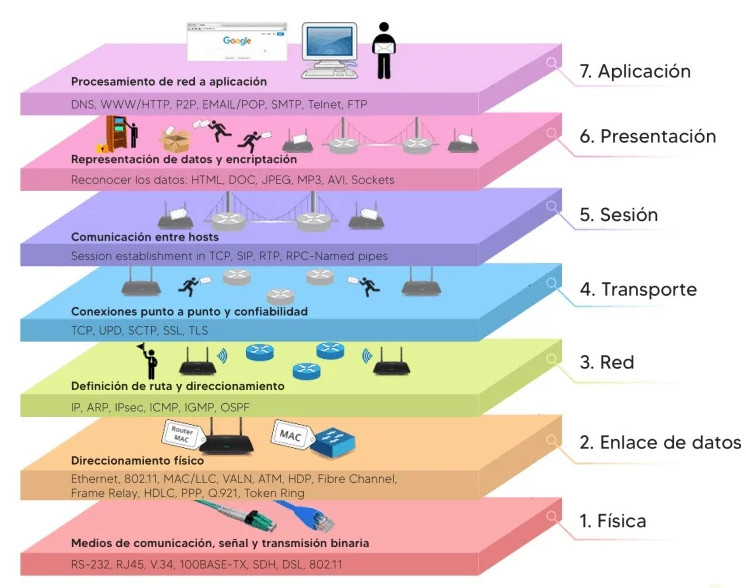
\includegraphics[scale=0.43]{Figura 4 - Modelo OSI.jpg}
\caption[Modelo OSI]{Modelo OSI. \footnotemark}
\label{fig:5}
\end{figure}
\footnotetext{Imagen tomada de: \url{https://platzi.com/clases/2225-redes/35587-modelo-osi/}}

A continuación se presentan en detalle las funciones de cada capa.

\begin{itemize}
	\item Capa 1 o física: define todas las especificaciones eléctricas y físicas de los dispositivos.
	\item Capa 2 o de enlace de datos: proporciona direccionamiento físico y procedimientos de acceso a medios.
	\item Capa 3 o de red: se encarga del direccionamiento lógico y el dominio del enrutamiento.
	\item Capa 4 o de transporte: proporciona transporte confiable y control del flujo a través de la red.
	\item Capa 5 o de sesión: establece, administra y finaliza las conexiones entre las aplicaciones locales y las remotas.
	\item Capa 6 de presentación: transforma el formato de los datos y proporciona una interfaz estándar para la capa de aplicación.
	\item Capa 7 o de aplicación: responsable de los servicios de red para las aplicaciones.
\end{itemize}

\subsection{Protocolo HTTP}

El protocolo de transferencia de hipertexto, conocido como HTTP (en inglés \textit{Hypertext Transfer Protocol}), es el protocolo de comunicación que permite las transferencias de información a través de archivos como XML y HTML entre otros. Está orientado a transacciones y sigue el esquema petición y respuesta entre un cliente y un servidor. El cliente realiza una petición enviando un mensaje con un formato determinado, al servidor. El servidor le envía un mensaje de respuesta con la información solicitada o un mensaje de error. \citep{9}

Los mensajes HTTP son en texto plano y tienen la siguiente estructura:

\begin{itemize}
	\item Línea inicial.
	\item Cabecera.
	\item Cuerpo.
\end{itemize}

En la línea inicial se envían las peticiones con el método hacia el servidor o las respuestas con el código devueltas hacia el navegador. Los métodos más comunes, y utilizados en el proyecto, son:

\begin{itemize}
	\item GET: solicita una representación del recurso especificado.
	\item POST: envía datos para que sean procesados por el recurso identificado en la URL de la línea de petición.
	\item PUT: envía datos al servidor. La diferencia con POST es que este está orientado a la creación de nuevos contenidos, mientras que PUT está orientado a la actualización de los mismos.
	\item DELETE: Borra el recurso especificado.
\end{itemize}

\subsection{Protocolo MQTT}

El protocolo de transporte de telemetría de colas de mensajes, conocido como MQTT (en inglés \textit{Message Queue Telemetry Transport}) es uno de los más utilizados y difundidos en IoT (sigla para Internet de las cosas, o \textit{Internet of things} en inglés). Es un protocolo de capa de aplicación, posee una topología de estrella y sus mensajes se transmiten como colas de publicación/suscripción.

El nodo central de su topología se llama \textit{broker} y es al cual se conectan los clientes remotos. El \textit{broker} se encarga de gestionar la red, recibir todos los mensajes de los clientes y redirigirlos hacia los clientes de destino. Un cliente es cualquier dispositivo que pueda interactuar con el \textit{broker} para enviar y recibir mensajes. Puede ser un sensor de IoT en campo o una aplicación en un centro de datos que procesa datos provenientes de los sensores. Cualquier cliente puede publicar o suscribirse a \textit{topics} (temas) para acceder a la información. Un \textit{topic} se representa mediante una cadena de texto con una estructura jerárquica. Cada jerarquía se separa con el caracter "/".

La finalidad de MQTT es minimizar el uso recursos en los dispositivos (CPU, RAM, ROM), ser confiable y ofrecer distintos niveles calidad del servicio. Consume un ancho de banda relativamente bajo y mantiene una conexión continua entre el broker y los clientes. Generalmente se suele usar este protocolo como nexo entre los dispositivos de campo con elementos típicos de software como servidores webs, bases de datos o herramientas de análisis. En la figura \ref{fig:6} se puede ver una arquitectura básica de conexión MQTT. \citep{10}

\begin{figure}[h]
\centering
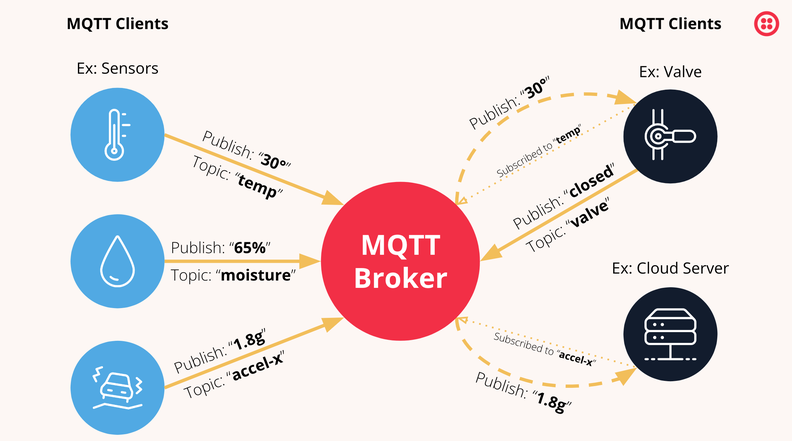
\includegraphics[scale=0.96]{Figura 5 - Arquitectura MQTT.png}
\caption[Arquitectura MQTT]{Arquitectura MQTT. \footnotemark}
\label{fig:6}
\end{figure}
\footnotetext{Imagen tomada de: \url{https://www.twilio.com/blog/what-is-mqtt}}

Para reforzar la seguridad en la comunicación mediante MQTT, se pueden proteger los datos mediante el uso de usuario y contraseña, o con cifrado de capa de sockets seguros, conocidos como SSL (en inglés \textit{Secure sockets layer}). La capa de transporte segura, o TLS, es una versión actualizada y más segura de SSL, y es por esto que en la actualidad se refiere a SSL/TLS como sinónimos.

\subsubsection{Protocolos SSL y TLS}

SSL y TLS son protocolos criptográficos, que proporcionan comunicaciones seguras por una red. Se usa criptografía asimétrica para autentificar a la contraparte con quien se están comunicando, y para intercambiar una llave simétrica. Esta sesión es luego usada para cifrar el flujo de datos entre las partes. Esto permite la confidencialidad del dato/mensaje, códigos de autenticación de mensajes para integridad y como un producto lateral, autenticación del mensaje. 

Antes de que un cliente y el servidor pueden empezar a intercambiar información protegida por TLS, deben intercambiar en forma segura o acordar una clave de cifrado y una clave para usar cuando se cifren los datos. Existen varios métodos utilizados para el intercambio y acuerdo de claves. \citep{11}

\section{Componentes de hardware}

\subsection{Raspberry Pi}

Las placas Raspberry Pi son computadoras de placa simple (en inglés \textit{single board computer} o su sigla SBC). Actualmente en el mercado existen distintas marcas y variantes de este tipo de placas, siendo elegidas tanto como computadoras de escritorio como para algunas aplicaciones específicas. A continuación se describen las principales características de la familia Raspberry Pi.

\begin{itemize}
	\item Posee puertos y entradas, permitiendo conectarla dispositivos periféricos como una pantalla táctil, un teclado e incluso un televisor.
	\item Contiene un procesador gráfico integrado, lo que permite la reproducción de vídeo, incluso en alta definición.
	\item Permite la conexión a la red a través del puerto de Ethernet, y algunos modelos permiten conexión Wi-Fi y Bluetooth.
	\item Consta de una ranura microSD que permite instalar, a través de una tarjeta de memoria, sistemas operativos.
\end{itemize}

El diseño de la Raspberry Pi fue evolucionando con el correr del tiempo. En la actualidad se encuentran los modelos Raspberry Pi 4 y Raspberry Pi 400, siendo los más modernos y robustos lanzados por la marca. La familia de Raspberry Pi 4 cuenta con 4 modelos de placa con distinta capacidad de memoria RAM, yendo desde 1 GB hasta 8 GB. La Raspberry Pi 400 es una variante de la Raspberry Pi la Raspberry Pi 400. También existen modelos más pequeños y limitados en recursos diseñados para otro tipo de aplicaciones.

En la figura \ref{fig:7} se pueden ver los modelos Raspberry Pi 4 y Raspberry Pi 400.

\begin{figure}[h]
\centering
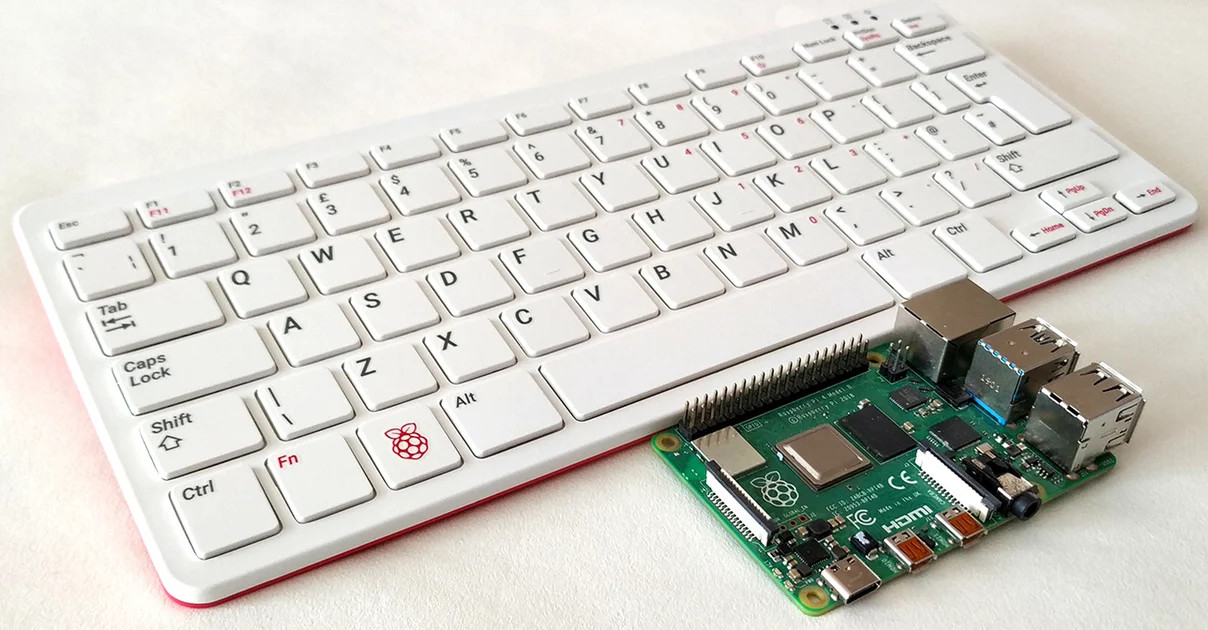
\includegraphics[scale=0.23]{Figura 6 - Raspberry.jpg}
\caption[Raspberry Pi]{Raspberry Pi 4 y Raspberry Pi 400. \footnotemark}
\label{fig:7}
\end{figure}
\footnotetext{Imagen tomada de: \url{https://all3dp.com/2/raspberry-pi-400-vs-raspberry-pi-4-differences/}}

Algunas de las funciones y aplicaciones más comunes de este tipo de computadoras se describen a continuación.

\begin{itemize}
	\item Navegar en la red, utilizar aplicaciones de oficina para la edición de documentos y emplearla como si fuese una computadora de escritorio.
	\item Crear un centro multimedia y ver los archivos guardados en su memoria.
	\item Se puede utilizar como un servidor privado dentro de una red local.
	\item Conectar los puertos del microprocesador desde un conector de 40 pines a distintos circuitos y dispositivos.
\end{itemize}

\subsection{Sistema en chip}

Un sistema en chip o SoC (del inglés \textit{system on a chip}) es aquel dispositivo que posee integrados todos o gran parte de los módulos que componen un sistema informático o electrónico en un único circuito integrado o chip. El diseño de estos sistemas puede estar basado en circuitos de señal digital, señal analógica y a menudo módulos o sistemas de radiofrecuencia. Un ámbito común de aplicación de la tecnología SoC son los sistemas embebidos.

Un SoC estándar está constituido por: \citep{12}

\begin{itemize}
	\item Un microcontrolador con el núcleo de la CPU. Algunos son construidos con microprocesadores dotados de varios núcleos.
	\item Módulos de memoria ROM (memoria de sólo lectura), RAM (memoria de acceso aleatorio), EEPROM (memoria de sólo lectura programable y borrable electrónicamente) y Flash (memorias de acceso muy rápido).
	\item Generadores de frecuencia fija.
	\item Componentes periféricos como contadores, temporizadores y relojes en tiempo real o RTC (en inglés \textit{real time clock}).
	\item Controladores de comunicación con interfaces externas normalmente estándar como USB, Ethernet, UART, o SPI.
	\item Controladores de interfaces analógicas, incluyendo conversores analógico a digital (ADC) y digital a analógico (DAC).
	\item Reguladores de voltaje y circuitos de gestión eficaz de la energía.
\end{itemize}

\subsubsection{Familia ESP32}

ESP32 es la denominación de una familia de chips SoC de bajo costo y consumo de energía, con tecnología Wi-Fi y Bluetooth de modo dual integrada. El ESP32 emplea un microprocesador Tensilica Xtensa LX6 en sus variantes de simple y doble núcleo e incluye interruptores de antena, balun de radiofrecuencia, amplificador de potencia, amplificador receptor de bajo ruido, filtros y módulos de administración de energía. El ESP32 fue creado y desarrollado por Espressif Systems.

En la figura \ref{fig:8} se pueden ver algunos de los módulos de desarrollo que contienen ESP32.

\begin{figure}[h]
\centering
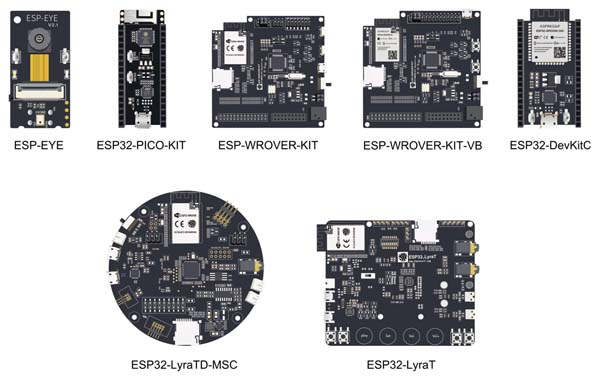
\includegraphics[scale=0.6]{Figura 7 - Familia ESP32.jpg}
\caption[Familia ESP32]{Módulos de la familia ESP32. \footnotemark}
\label{fig:8}
\end{figure}
\footnotetext{Imagen tomada de: \url{https://www.electrodaddy.com/esp32/}}

\section{Herramientas de software}
\subsection{Visual studio code}

Visual Studio Code es un editor de código fuente desarrollado por Microsoft para múltiples sistemas operativos. Incluye soporte para la depuración, control integrado de Git, resaltado de sintaxis, finalización inteligente de código, fragmentos y refactorización de código. Es personalizable y tiene la posibilidad de instalar extensiones para agregar lenguajes, depuradores y herramientas para el desarrollo de código. Es gratuito y de código abierto, aunque la descarga oficial está bajo software privativo e incluye características personalizadas por Microsoft.

Algunos de los lenguajes de programación que es capaz de manejar son: C, C++, Dockerfile, Git-commit, HTML, JSON, Java, Javascript, PHP, Python, Ruby, Rust, SQL, Shell script, TypeScript y Visual Basic entre otros.

\subsection{Marco de desarrollo ESP}

El marco de desarrollo de ESP, o ESP-IDF (en inglés \textit{ESP IoT Development Framework}) es un entorno completo de programación para desarrollar sistemas embebidos para dispositivos ESP. Es desarrollado por Espressif y se puede descargar como una extensión de Visual studio code. El lenguaje de programación es C e incluye herramientas para cargar el código desarrollado al chip y depurar el programa en tiempo real.

El lenguaje C es un lenguaje de programación de propósito general de tipos de datos estáticos, débilmente tipado. Dispone de las estructuras típicas de los lenguajes de alto nivel pero, a su vez, dispone de construcciones del lenguaje que permiten un control a bajo nivel. Uno de los objetivos de diseño del lenguaje C es que solo sean necesarias unas pocas instrucciones en lenguaje máquina para traducir cada elemento del lenguaje, sin que haga falta un soporte intenso en tiempo de ejecución. \citep{13}

\subsection{Lenguajes JavaScript y TypeScript}

JavaScript (abreviado comúnmente JS) es un lenguaje de programación interpretado. Se define como orientado a objetos, basado en prototipos, imperativo, débilmente tipado y dinámico. Se utiliza principalmente del lado del cliente, implementado como parte de un navegador web permitiendo mejoras en la interfaz de usuario y páginas web dinámicas y JavaScript del lado del servidor. Todos los navegadores modernos interpretan el código JavaScript integrado en las páginas web. Para interactuar con una página web se provee al lenguaje JavaScript de una implementación del modelo de objeto de documento, o DOM (en inglés \textit{Document Object Model}). Javascript es el único lenguaje de programación que entienden de forma nativa los navegadores. \citep{14}

TypeScript es un lenguaje de programación libre y de código abierto desarrollado y mantenido por Microsoft. Es un superconjunto de JavaScript, que esencialmente añade tipos estáticos y objetos basados en clases. Es usado para desarrollar aplicaciones JavaScript que se ejecutarán en el lado del cliente o del servidor, o extensiones para programas. Extiende la sintaxis de JavaScript, por tanto cualquier código JavaScript existente debería funcionar sin problemas. Está pensado para grandes proyectos, los cuales a través de un compilador de TypeScript se traducen a código JavaScript original. \citep{15}

\subsection{Angular y Ionic}

Angular es un marco de desarrollo (\textit{framework} en inglés) de ingeniería de software de código abierto mantenido por Google, que sirve para desarrollar aplicaciones web de estilo aplicación de una sola página (en inglés \textit{single page application} o SPA) y aplicación web progresiva (en inglés \textit{progressive web app} o PWA). Sirve tanto para versiones móviles como de escritorio. Ofrece soluciones robustas, escalables y optimizadas para lograr un estilo de codificación homogéneo y de gran modularidad. Su desarrollo se realiza por medio de TypeScript o JavaScript. En este último se ofrecen diversas herramientas adicionales al lenguaje como tipado estático o decoradores. \citep{16}

El marco de desarrollo Ionic es un kit de desarrollo de software (en inglés \textit{software development kit} o SDK) de frontend de código abierto para desarrollar aplicaciones híbridas basado en tecnologías web (HTML, CSS y JS). Es decir, un \textit{framework} que nos permite desarrollar aplicaciones multiplataforma desde una única base de código. Posee la capacidad de integrarse con otros marcos populares como Angular, React y Vue. Su principal característica es que permite desarrollar y desplegar aplicaciones híbridas, que funcionan en múltiples plataformas, como iOS nativo, Android, escritorio y la web (como una aplicación web progresiva) con una única base de código. \citep{17}

\subsection{Contenedores con Docker}

Los contenedores son una forma de virtualización del sistema operativo. Un solo contenedor se puede usar para ejecutar cualquier aplicación, desde un microservicio o un proceso de software a una aplicación de mayor tamaño. Dentro de un contenedor se encuentran todos los ejecutables, el código binario, las bibliotecas y los archivos de configuración necesarios. Sin embargo, en comparación con los métodos de virtualización de máquinas o servidores, los contenedores no contienen imágenes del sistema operativo. Esto los hace más ligeros y portátiles, con una sobrecarga significativamente menor. En implementaciones de aplicaciones de mayor tamaño, se pueden poner en marcha varios contenedores como uno o varios clústeres de contenedores. Estos clústeres se pueden gestionar mediante un orquestador de contenedores, como Kubernetes o Docker Compose. \citep{18}

Docker es un proyecto de código abierto que automatiza el despliegue de aplicaciones dentro de contenedores de software, proporcionando una capa adicional de abstracción y automatización de virtualización de aplicaciones en múltiples sistemas operativos. Usar Docker para crear y gestionar contenedores puede simplificar la creación de sistemas altamente distribuidos, permitiendo que múltiples aplicaciones, las tareas de los trabajadores y otros procesos funcionen de forma autónoma en una única máquina física o en varias máquinas virtuales. \citep{19} En la figura \ref{fig:9} se puede ver de forma gráfica el funcionamiento de un contenedor Docker.

\begin{figure}[h]
\centering
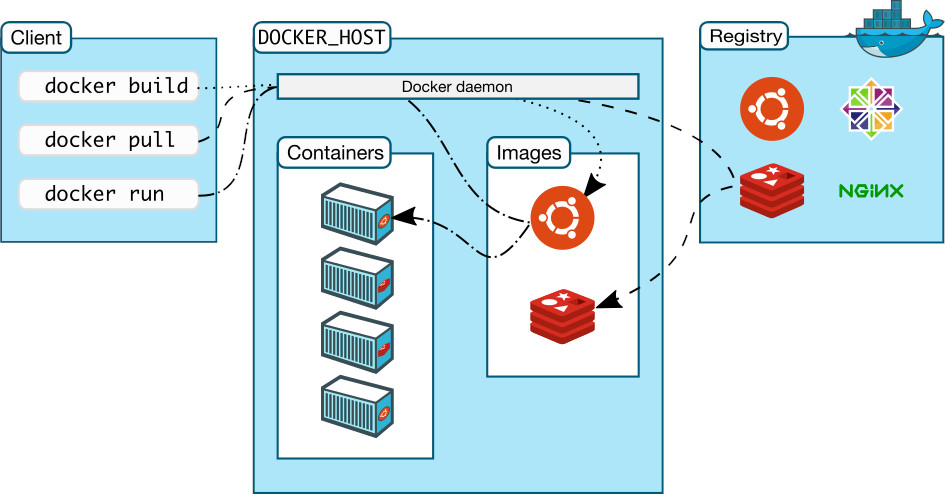
\includegraphics[scale=0.4]{Figura 8 - Docker.jpg}
\caption[Docker]{Contenedor Docker. \footnotemark}
\label{fig:9}
\end{figure}
\footnotetext{Imagen tomada de: \url{https://algodaily.com/lessons/what-is-a-container-a-docker-tutorial}}


Docker Compose es una herramienta para definir y ejecutar aplicaciones Docker de varios contenedores. Con Compose, utiliza un archivo YAML para configurar los servicios de su aplicación. Luego, con un solo comando, se crean e inician todos los servicios desde su configuración. Tiene comandos para gestionar todo el ciclo de vida de tu aplicación: \citep{20}

\begin{itemize}
	\item Iniciar, detener y reconstruir servicios.
	\item Ver el estado de los servicios en ejecución.
	\item Transmitir la salida del registro de los servicios en ejecución.
	\item Ejecutar un comando único en un servicio.
\end{itemize}